%!TEX root = ../per_st_tk.tex

\begin{frame}{Cup-$i$ coproducts}
	\pause
	We need \colorit{explicit} maps
	\[
	\Delta_i \colon \gchains(X) \to \gchains(X)^{\otimes 2}
	\quad \text{satisfying} \quad
	\partial \Delta_{i} = \big(1 \pm T \big) \Delta_{i-1}
	\]

	\pause\bigskip\smallskip
	Then, the \colorit{product} is
	\[
	\begin{split}
		H^\bullet(X) \ot H^\bullet(X) &\to H^\bullet(X) \\
		[\alpha] \ot [\beta] &\mapsto \big[ (\alpha \otimes \beta) \Delta_0(-) \big]
	\end{split}
	\]

	\smallskip\pause
	and the $k^\th$ \colorit{Steenrod square}
	\[
	\begin{split}
		\Sq^k \colon H^\bullet(X; \Ftwo) &\to H^\bullet(X; \Ftwo) \\
		[\alpha] &\mapsto \big[ (\alpha \otimes \alpha) \Delta_{\bars{\alpha}-k}(-) \big]
	\end{split}
	\]
\end{frame}

\begin{frame}{A new description of Steenrod's construction}
	\pause
	\colorit{Notation.}
	\vspace*{-10pt}
	\begin{align*}
		&\forall n,q \in \N,
		\quad \rP_q^n = \set[\big]{U \subseteq \{0, \dots, n\} : \bars{U} = q} \\
		&\forall U = \{u_1 < \dots < u_q\} \in \rP_q^n,
		\quad d_U = d_{u_1} \dotsm \, d_{u_q}
	\end{align*}

	\pause
	\colorit{Definition (Med.)} \\
	For a basis element $x \in \gchains_m(X, \Ftwo)$
	\[
	\textstyle \Delta_i(x) = \sum d_{U^0}(x) \otimes d_{U^1}(x)
	\]
	where the sum is over $\rP^n_{n-i}$ and
	\begin{equation*} \label{e:partition subsets}
		U^0 = \{u_j \in U\mid u_j \equiv j \text{ mod } 2\}, \qquad
		U^1 = \{u_j \in U\mid u_j \not\equiv j \text{ mod } 2\}.
	\end{equation*}

	\pause\medskip
	\colorit{Theorem (Med.)} \\
	All cup-$i$ constructions in the literature are equal up isomorphism:
	\vskip -7.5pt
	\[
	\triangle \sim \triangle^\prime \iff \forall i \in \N, \ \triangle_i = \triangle_i^\prime \ \vee \, \triangle_i = T \triangle_i^\prime.
	\]
	\vskip -3pt
	(Proven via an axiomatic characterization.)
\end{frame}

\begin{frame}{Fast computation of Steenrod squares}
	\pause
	Comparing to SAGE: (algorithm based on EZ-AW contraction)

	\smallskip\pause
	\colorit{$\Sq^1$} on \colorit{$\Sigma^i\R P^2$} ($i^\th$ suspension of the real projective plane)

	\medskip
	\includegraphics[width=\textwidth]{aux/comp_sus_rp2.pdf}
\end{frame}

\begin{frame}{Steenrod squares for simplicial complexes}
	\begin{algorithm} [H]
	\KwIn{$A = \{a_1, \dots, a_m\} \subseteq X_n$}
	$B = \emptyset$ \\
	\ForAll{$a_i\ \mathrm{and}\ a_j\ \mathrm{with}\ i < j$}
	{
		$a_{ij} = a_i \cup a_j$ \\
		\If{$a_{ij} \in X_{n+k}$}
		{
			$\overline{a}_i = a_i \setminus a_j$\ ;\ \
			$\overline{a}_j = a_j \setminus a_i$\ ;\ \
			$\overline{a}_{ij} = \overline{a}_i \cup \overline{a}_j$ \\
			$index \colon \overline{a}_{ij} \to \{0,1\}$ \\
			\ForAll {$v \in \overline{a}_{ij}$}
			{
				$p = \mathrm{position\ of\ } v \mathrm{\ in\ } a_{ij}$\ ;\ \
				$\overline{p} = \mathrm{position\ of\ } v \mathrm{\ in\ } \overline{a}_{ij}$\\
				$index(v) = {p}\, +\, \overline{p}\ \ \mathrm{residue\ mod}\ 2$
			}
			\If{\hspace*{3pt}$index(\overline{a}_i) \xor index(\overline{a}_j)$ = $\{0,1\}$}
			{$B = B \xor \{a_{ij}\}$}
		}
	}
	\KwOut{$B$}
\end{algorithm}
\end{frame}

\begin{frame}{Points clouds and multi-scale approximation}
	\pause
	Data sets are often encountered as point clouds in $\R^n$.

	\pause
	\begin{center}
		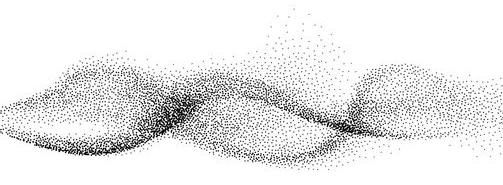
\includegraphics[scale=.4]{aux/point_cloud_cropped}
	\end{center}

	\pause
	Their underlying probability distribution is concentrated on a subspace.

	\medskip\pause
	Use \colorit{distance parameter} to approximate it with simplicial complexes.
	\medskip
	\begin{center}
		\includegraphics[scale=.7]{aux/vietoris-rips}
	\end{center}

	\vskip-15pt
	\[
	X_{0} \subset X_{1} \subset\dots\subset X_{n}
	\]
\end{frame}

\begin{frame}{Persistence homology}
	\pause
	Applying a homology functor (over a field)
	\[
	H_d(X_0) \to H_d(X_1) \to\dots\to H_d(X_n)
	\]
	get a \colorit{persistence module}, i.e. a diagram of vector spaces.

	\pause\bigskip
	The way dimensions fit together defines the \colorit{barcode}.
	\begin{center}
		\includegraphics[scale=.7]{aux/vietoris-rips}
		\includegraphics[scale=.6]{aux/betti}
	\end{center}

	\pause\smallskip
	\colorit{Stability}: The passage from point clouds to barcodes is Lipschitz
	\[
	d_{GH}(\fX, \fX') \leq c \cdot d_{BN}(B_{\fX}, B_{\fX'}).
	\]

	\pause
	\colorit{Computability}: Based on matrix reduction algorithms
	\[
	\sim O(n^3).
	\]
\end{frame}

\begin{frame}{Dualities}
	\pause
	The Betti barcodes of

	\medskip
	\quad Abs Hom\phantom{co} \qquad $H_d(X_0) \to H_d(X_1) \to\dots\to H_d(X_n)$

	\medskip
	\quad Abs coHom \!\qquad $H^d(X_0) \leftarrow H^d(X_1) \leftarrow\dots\leftarrow H^d(X_n)$

	\medskip
	\quad Rel Hom\phantom{co} \qquad $H_d(X_n,X_0) \leftarrow H_d(X_n,X_1) \leftarrow\dots\leftarrow H_d(X_n,X_n)$

	\medskip
	\quad Rel coHom \!\qquad $H^d(X_n,X_0) \to H^d(X_n,X_1) \to\dots\to H^d(X_n,X_n)$

	\medskip
	provide \colorit{equivalent} information.

	\pause\medskip
	But \colorit{cohomology} has performance and theoretical \colorit{advantages}.
\end{frame}

\begin{frame}[fragile]{Steenrod barcodes}
	\pause
	Given a filtered simplicial complex $X$
	\[
	X_0 \to X_1 \to \cdots \to X_n.
	\]

	\pause
	Cohomology induces a \colorit{persistent module}, its \colorit{barcode} is a summary of how Betti numbers are consecutively shared.\\

	\smallskip
	\phantom{A cohomology operation induces an endomorphism}
	\[
	\begin{tikzcd}[column sep = 15]
		H^\bullet(X_n; \Ftwo) \arrow[r] & \cdots \arrow[r] & H^\bullet(X_{n-1}; \Ftwo) \arrow[r] & H^\bullet(X_0; \Ftwo) \\
		\phantom{H^\bullet(X_n; \Ftwo)} \arrow[u, "\phantom{\Sq^k}", phantom] & \phantom{\cdots} & \phantom{H^\bullet(X_{n-1}; \Ftwo)} & \phantom{H^\bullet(X_0; \Ftwo)} \arrow[u, "\phantom{\Sq^k}", phantom] \phantom{.}
	\end{tikzcd}
	\]
\end{frame}

\begin{frame}[fragile]{Steenrod barcodes}
	Given a filtered simplicial complex $X$
	\[
	X_0 \to X_1 \to \cdots \to X_n.
	\]
	Cohomology induces a \colorit{persistent module}, its \colorit{barcode} is a summary of how Betti numbers are consecutively shared.

	\smallskip
	A cohomology operation induces an \colorit{endomorphism}
	\[
	\begin{tikzcd}[column sep = 15]
	H^\bullet(X_n; \Ftwo) \arrow[r] & \cdots \arrow[r] & H^\bullet(X_{n-1}; \Ftwo) \arrow[r] & H^\bullet(X_0; \Ftwo) \\
	H^\bullet(X_n; \Ftwo) \arrow[u, "\Sq^k"] \arrow[r] & \cdots \arrow[r] & H^\bullet(X_{n-1}; \Ftwo) \arrow[u, "\Sq^k"] \arrow[r] & H^\bullet(X_0; \Ftwo) \arrow[u, "\Sq^k"].
	\end{tikzcd}
	\]

	\pause
	\colorit{Definition (Lupo--Med.--Tauzin)} \\
	The \colorit{$\Sq^k$-barcode} of $X$ is defined as the barcode of $\mathrm{img}\ \Sq^k$.

	\pause\medskip
	\colorit{Theorem (Ling Zhou--Med.--M\'emoli)} \\
	These barcodes are stable.
\end{frame}

\begin{frame}{Example $\Sq^2$} \pause
	Filtrations of the cone on the suspension of $S^2 \vee S^4$ and $\bC \rP^2$.

	\pause
	\begin{figure}
		\centering
		\begin{subfigure}[b]{0.49\textwidth}
			\centering
			\includegraphics[width=\textwidth]{aux/s2_s4.pdf}
			\caption{$\mathrm C\,\Sigma(S^2 \vee S^4)$}
			\label{f:s2_s4}
		\end{subfigure}
		\begin{subfigure}[b]{0.49\textwidth}
			\centering
			\includegraphics[width=\textwidth]{aux/cp2.pdf}
			\caption{$\mathrm C\,\Sigma\,\bC\rP^2$}
			\label{f:cp2}
		\end{subfigure}
	\end{figure}
\end{frame}

\begin{frame}{Algorithm}
	\pause
	It has three steps:

	\begin{enumerate}
		\pause\bigskip
		\item Usual reduction applied to the anti-transposed boundary $M$ yielding
		\[
		R = M V
		\]
		where $R$ is reduced and $V$ is invertible.

		\pause\bigskip
		\item Read off cohomology representatives and apply the new $\Sq^k$ algorithm to create a matrix $Q^k$ with the resulting representatives.

		\pause\bigskip
		\item Using that $R$ is made of generating coboundaries, apply a reduction algorithm to $Q^k$ with respect to $R$ recording the rank of $Q_{\leq j}^k$.
	\end{enumerate}
\end{frame}

%\begin{frame}{Third step}
%	\begin{algorithm}[H]
	\KwIn{$R,\, Q^k$}
	Alive $= \{0, \dots, m\}$,
	Barcode $= \emptyset$ \\
	\For{$j = 0, \dots, m$}{
		$R_{\leq j} \mid Q^k_{\leq j} = \text{Reduce}\left( R_{\leq j} \mid Q^k_{\leq j} \right)$ \\
		\For{$i = 0, \dots, j$}{
			\If{$i \in \mathrm{Alive\ and\ } Q^k_i = 0$}{
				remove $i$ from Alive \\
				\If{$i <j $}{add $[m-j, m-i]$ to Barcode}
			}
		}
	}
	\For{$i \in \mathrm{Alive}$}{
		add $[-1, m-i]$ to Barcode
	}
	\KwOut{Barcode}
\end{algorithm}
%\end{frame}

\begin{frame}{\texttt{steenroder}}
	\pause
	With \textit{U. Lupo} and \textit{G.~Tauzin}

	\begin{center}
		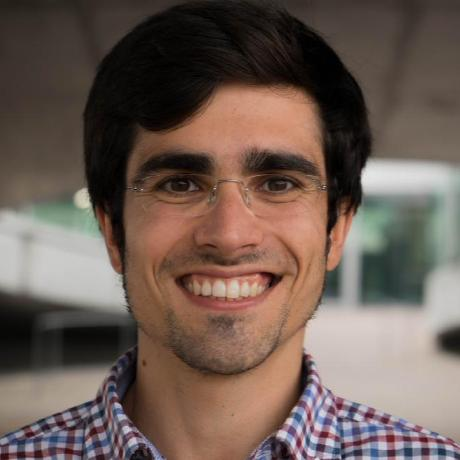
\includegraphics[scale=.2]{aux/umberto}
		\qquad
		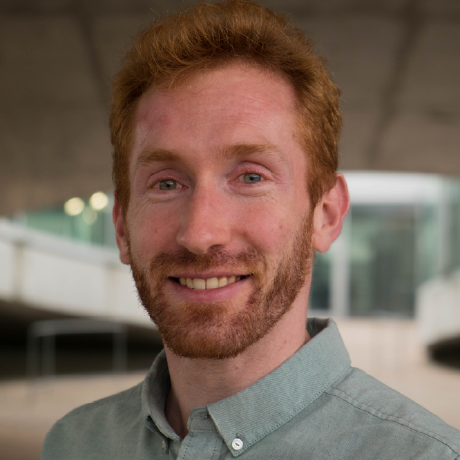
\includegraphics[scale=.2]{aux/guillaume}
	\end{center}

	from \colorit{\texttt{giotto-tda}}'s team we developed a Python package for this.

	\pause\smallskip
	It can easily installed via
	\begin{center}
		\texttt{python -m pip install -U steenroder}
	\end{center}

	and we accept contributions at
	\begin{center}
		\url{https://github.com/Steenroder/steenroder}
	\end{center}
\end{frame}

\begin{frame}{Space of conformations of $\mathrm{C_8H_{16}}$}
	\pause
	Points in $\R^{24}$ (positions of $8$ carbons in $\R^3$)

	\pause\medskip
	$H^1$ (green) and $H^2$ (blue) barcodes of (part of) this point cloud
	\includegraphics[width=\textwidth]{aux/molecule_top.pdf}

	\pause
	$\Sq^1$ barcode
	\includegraphics[width=\textwidth]{aux/molecule_bot.pdf}
	Consistent with a \colorit{Klein bottle}.
\end{frame}

%\begin{frame}{Space of conformations of $\mathrm{C_8H_{16}}$}
%	\pause
%	Points in $\R^{24}$ (positions of $8$ carbons in $\R^3$)
%
%	\pause\smallskip
%	Computing $\Sq^1$ barcode of a ``smooth component'' of this point cloud
%	\smallskip
%	\includegraphics[width=\textwidth]{aux/cyclo-octane_subsampled_absolute_barcodes.pdf}
%	Consistent with a \colorit{Klein bottle} component.
%\end{frame}

%\begin{frame}{Unicity of Steenrod's cup-$i$ construction}
%	\pause
%	\colorit{Theorem (Med.)} \\
%	All cup-$i$ constructions in the literature are equal up isomorphism:
%	\vskip -7.5pt
%	\[
%	\triangle \sim \triangle^\prime \iff \forall i \in \N, \ \triangle_i = \triangle_i^\prime \ \vee \, \triangle_i = T \triangle_i^\prime.
%	\]
%	\vskip -3pt
%	(Proven via an axiomatic characterization.)
%
%	\medskip\pause
%	\colorit{Theorem (Laplante-Anfossi--Med.--Vallette)} \\
%	Let $P \subset \R^n$ be an $n$-dim convex polytope.
%	A generic orthogonal ordered basis of $\R^n$ defines a cellular cup-$i$ construction $S^\infty \times P \to P \times P$.
%\end{frame}